\chapter*{Приложение А: Функциональная схема работы программы}
\addcontentsline{toc}{chapter}{Приложение А: Функциональная схема работы программы}

\begin{figure}[h!]
	\centering
	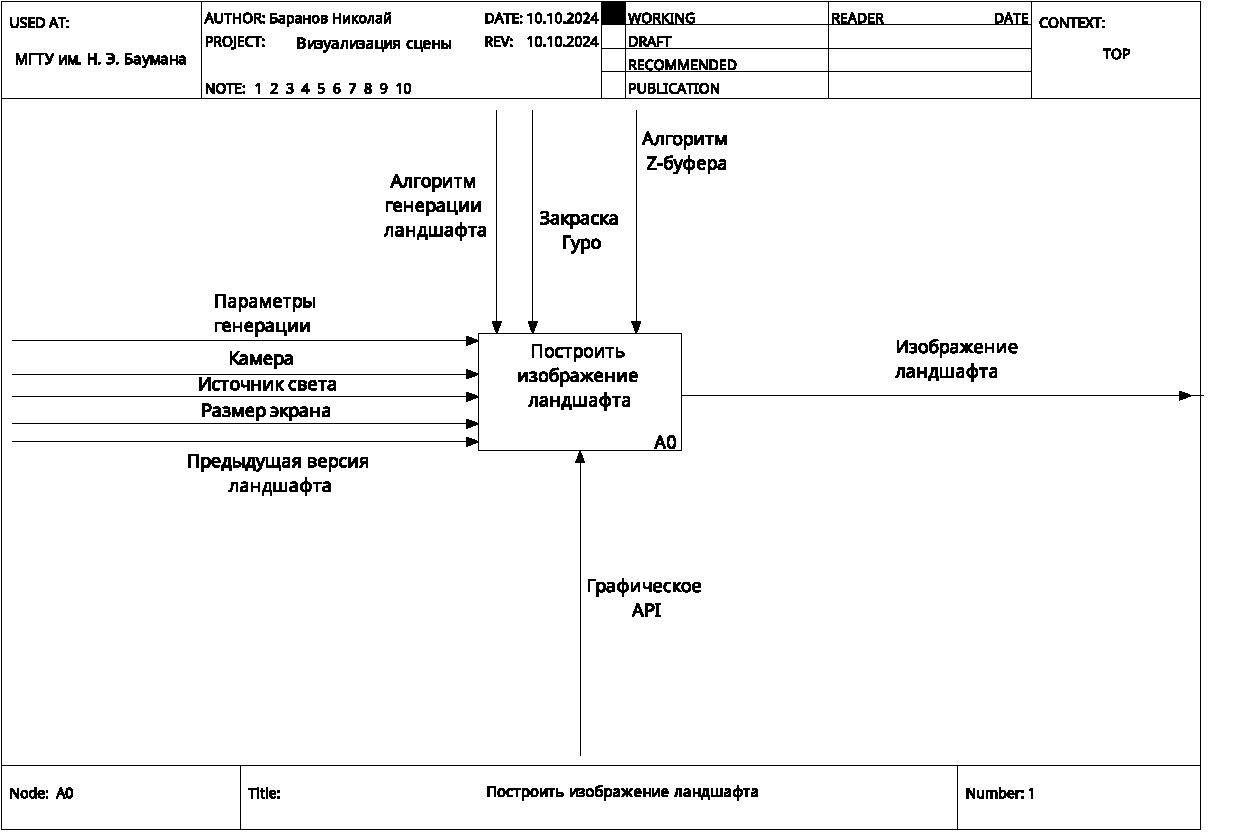
\includegraphics[width=0.9\textwidth]{tex_parts/01_A0.pdf}
	
	\text{Рисунок А.1 --- Верхний уровень функциональной схемы}
	%\caption[labelformat=empty]{\label{fig:first}}
\end{figure}

\begin{figure}[h!]
	\centering
	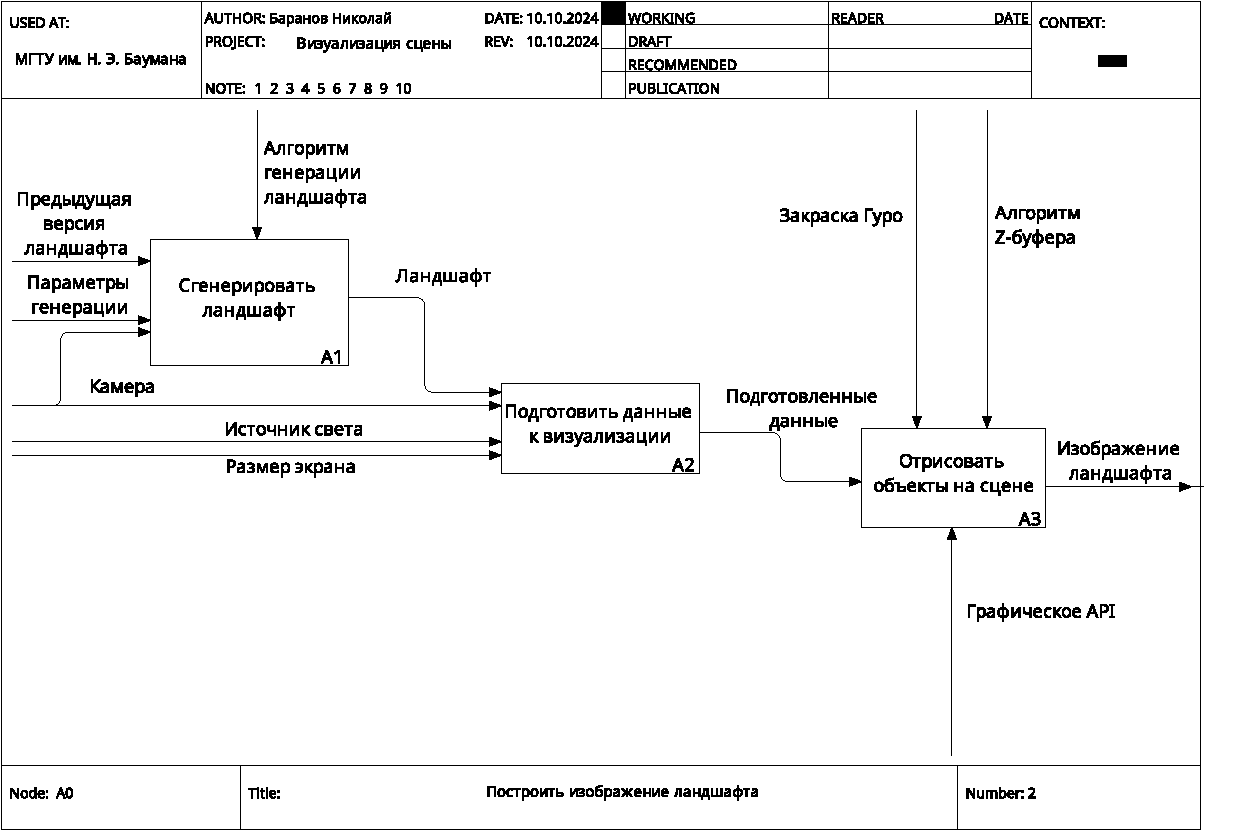
\includegraphics[width=0.9\textwidth]{tex_parts/02_A0.pdf}
	
	\text{Рисунок А.2 --- Декомпозиция уровня A0}
\end{figure}

\begin{figure}[h!]
	\centering
	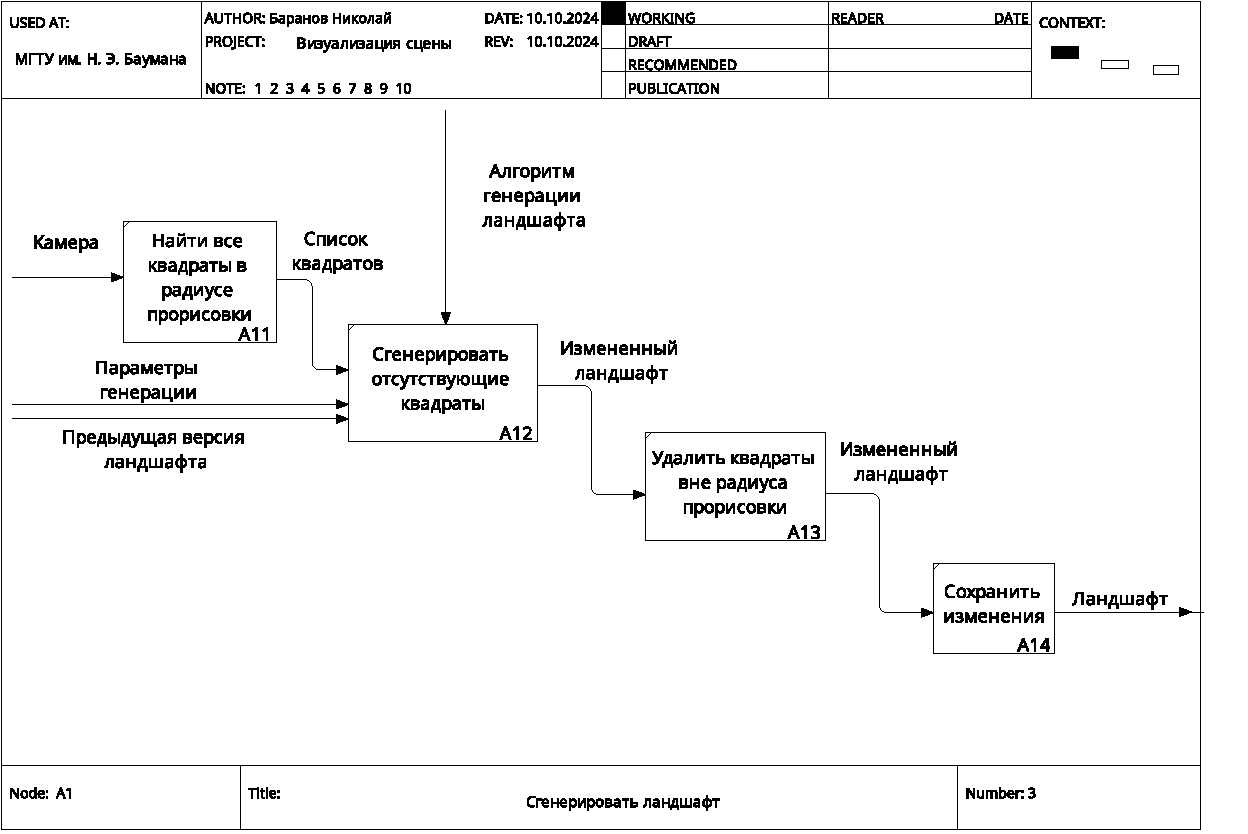
\includegraphics[width=0.9\textwidth]{tex_parts/03_A1.pdf}
		
	\text{Рисунок А.3 --- Декомпозиция уровня A1}
\end{figure}

\begin{figure}[h!]
	\centering
	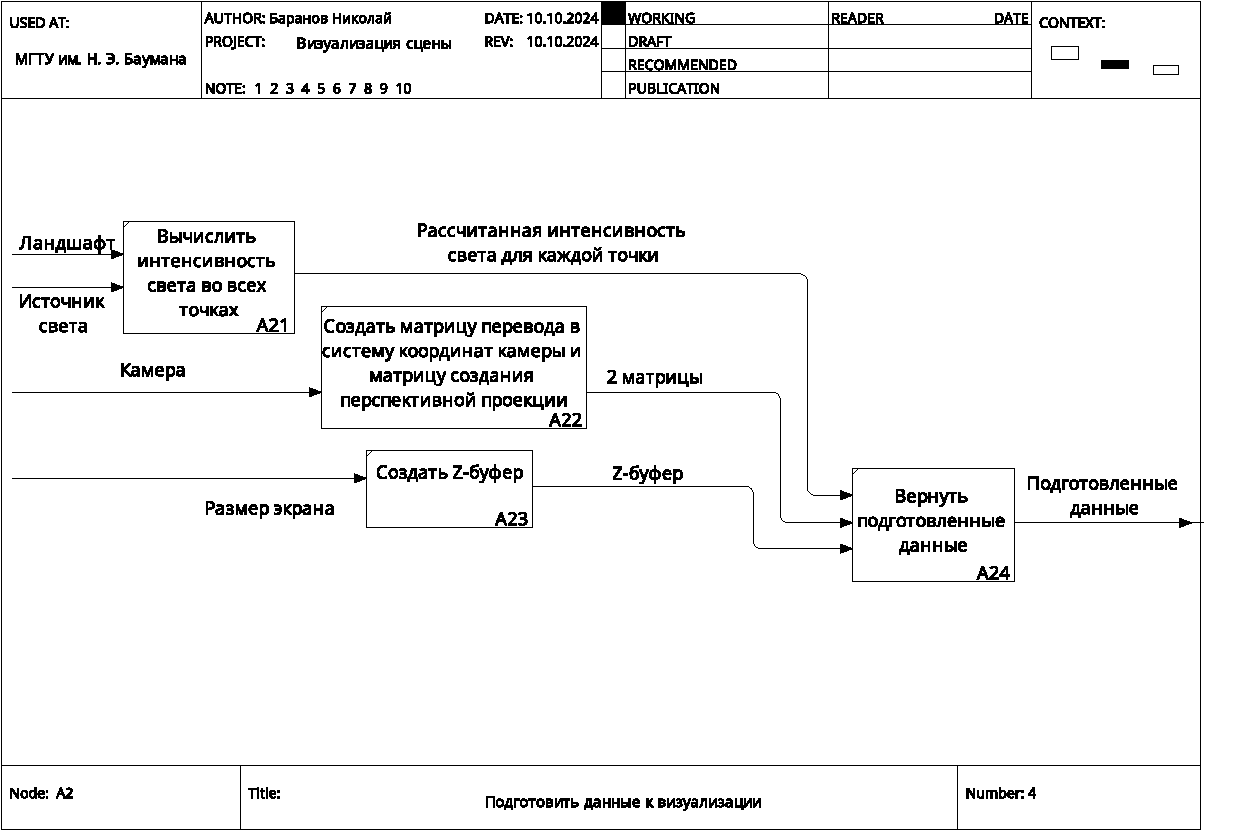
\includegraphics[width=0.9\textwidth]{tex_parts/04_A2.pdf}
		
	\text{Рисунок А.4 --- Декомпозиция уровня A2}
\end{figure}

\clearpage

\begin{figure}[H]
	\centering
	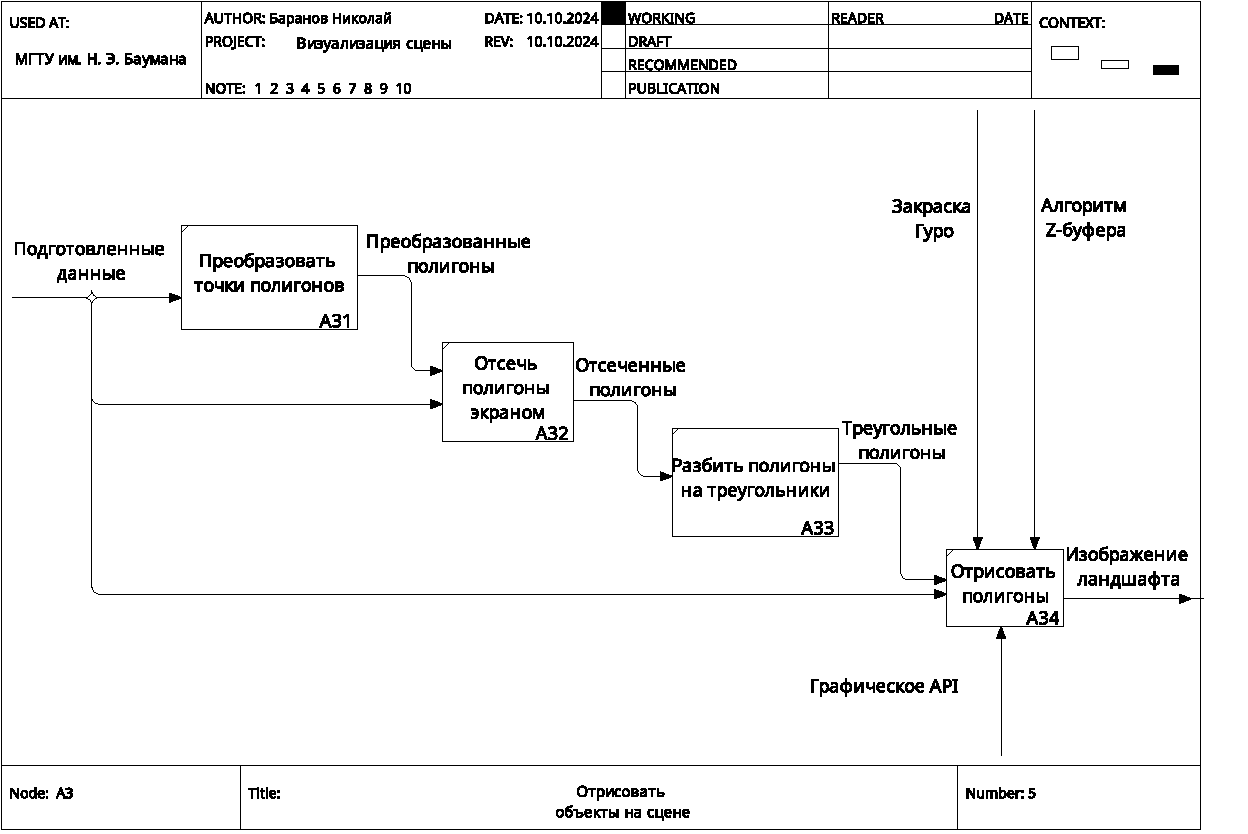
\includegraphics[width=0.9\textwidth]{tex_parts/05_A3.pdf}
		
	\text{Рисунок А.5 --- Декомпозиция уровня A3}
\end{figure}